\documentclass{article}
\usepackage[pdftex]{graphicx}
\usepackage{wrapfig}
\usepackage{enumerate}
\usepackage{hyperref}
\usepackage{fullpage}
\usepackage{cite}

\begin{document}

\title{CSE550 Problem Set 2: Paxos Design Document}
\author{Vincent Lee, Shumo Chu}
\date{\today}

\maketitle

\tableofcontents

%%%%%%%%%%%%%%%%%%%%%%%%%%%%%%%%%%%%%%%%%%%%%%%%%%%%%%%%%%%%%%%%%%%%%%%%%%%%%%
% Intro
%%%%%%%%%%%%%%%%%%%%%%%%%%%%%%%%%%%%%%%%%%%%%%%%%%%%%%%%%%%%%%%%%%%%%%%%%%%%%%

\section{Introduction}

In this document, we outline our software implementation of the Paxos consensus protocol explained in ``Paxos Made Simple'' by Leslie Lamport.
We present a high level software architecture, justify our design decisions, and explain any simplfying assumptions that we make to our design.
We then explain how to use our implementation, and any outstanding problems with our implementation.
A quick discussion of any interesting tidbits we encounter concludes the document.

%%%%%%%%%%%%%%%%%%%%%%%%%%%%%%%%%%%%%%%%%%%%%%%%%%%%%%%%%%%%%%%%%%%%%%%%%%%%%%
% Paxos Protocol Summary
%%%%%%%%%%%%%%%%%%%%%%%%%%%%%%%%%%%%%%%%%%%%%%%%%%%%%%%%%%%%%%%%%%%%%%%%%%%%%%

\section{Paxos Protocol}

The Paxos protocol is a consensus protocol designed to make forward progress even in the face of arbitrary server node and communication failures.
We interpret consensus to be defined as the following constraints:

\begin{enumerate}
\item One and only one value may be chosen per Paxos instance
\item The value must come from the set of proposals
\item Only the chosen values can propagate to learners
\end{enumerate}

The Paxos protocol consists of three classes of members: proposers, acceptors, and learners.
\begin{itemize}
\item Proposers are defined as entities that present proposals to acceptors.
\item Acceptors are defined as entities that are responsible for arbitrating whether a proposal is accepted or not.
\item Learners are defined as entities that are subscribed to a particular value that a consensus determines.
\end{itemize}

In any Paxos instance, in order to tolerate node failure, multiple proposers and acceptors participate in a Paxos instance.
A Paxos instance is resolved by the following a two phase protocol.

\subsection{Paxos Phase I}

In the first phase of the protocol, proposers create proposals with some associated monotonically increasing sequence number N and some instance number I. 
The sequence number is always larger than any previous sequence number the proposer has issued. 
A propose message is then sent to the set of acceptors with the sequence number chosen. 
When an acceptor receives a propose message, it compares the sequence number of the proposal to all previous sequence numbers it has seen.
If the sequence number received is less than any sequence number the acceptor has seen, the proposal is rejected and ignored.
A response message with the highest proposal seen and the value accepted is sent to the proposer instead.

If the sequence number received by the acceptor is greater than or equal to the prior sequence numbers observed by the acceptor, it ``promises'' to reject all messages less than the sequence number received from that point forward.
A response is issued with this ``promise'' to the original proposer.
Meanwhile, the original proposer wait until it receives responses from a majority of the acceptors it initially issued proposals to with sequence number N.
There are two cases at this stage of the protocol: the proposer gets messages from a majority of acceptors with a prepare acknowledgement for it's proposal number, 
or the proposer gets messages from a majority of acceptors with a prepare not acknowledgement (prepare NACK), the highest value each acceptor has accepted, and the value associated with this highest proposal number.
If the proposer gets a majority of previously accepted values from the acceptors it means that the instance may have already been resolved.
At this point the proposer will abandon its original proposal and propose this new value it received from a majority of acceptors and the proposal number.

\subsection{Paxos Phase II}

If a majority of messages are prepare NACKs with the same previously accepted value, the proposer abandons it's original proposal and changes the proposal value to the value and the proposal number to those in the prepare NACK message.
Once this resolution occurs, the proposer issues an accept request with the proposal number and value.
An acceptor will accept the proposal and chosen value if the highest sequence number is sees is still N, and reject the message otherwise.
Upon successful receipt of the accept message, messages are issued to all relevant learners with the value chosen and an accept message is issued to the original proposer.
If an acceptor rejects the accept request, the message will be discarded and no response will be issued.
A proposer knows its attempt to chose a value has failed if it does not receive responses from a majority of acceptors.

If at the end of a single iteration of this protocol, no value is ultimately chosen, the procedure is repeated with a higher sequence number of each node until a value is eventually chosen.
If the proposer is able to get a majority of accept requests, it knows that the Paxos instance has been resolved and moves on to the next one.
If during the first phase, the proposer had to abandon the original value, it tries to propose this value again in the next Paxos instance.

%%%%%%%%%%%%%%%%%%%%%%%%%%%%%%%%%%%%%%%%%%%%%%%%%%%%%%%%%%%%%%%%%%%%%%%%%%%%%%
% Implementation Details
%%%%%%%%%%%%%%%%%%%%%%%%%%%%%%%%%%%%%%%%%%%%%%%%%%%%%%%%%%%%%%%%%%%%%%%%%%%%%%

\section{Paxos Implementation of Lock Service}

Our design leverages the Paxos algorithm to implement an ordering of commands for a simple lock service.
Issuable commands in this service are $lock(x)$ and $unlock(x)$ where $x$ is an integer.
The end goal of this service is to provide consensus upon a series of commands in which locks are resolved in a valid order.
The state machine in this service is defined to be the state of the locks and is replicated across servers for resilience to failure.
Each instance of the Paxos protocol resolves exactly one command to be issued for that instance.
Instances are numbered in monotonically increasing order and correlate to sequence in which the $lock(x)$ and $unlock(x)$ commands are issued.

\subsection{Simplifying Assumptions}

We assume the same assumptions about the distributed system model as originally proposed in the Paxos paper. Namely, we assume the following:

\begin{enumerate}
\item No Byzantine failures will occur.
\item All entities in the distributed system operate asynchronously at arbitrary speed
\item Any node that fails in the system will observe fail-stop behavior
\item Messages at any phase during the protocol can be dropped, reordered, or duplicated
\end{enumerate}

We also make the following assumptions to simplify our implementation of the Paxos algorithm:

\begin{enumerate}
\item Any nodes that experience a failure will permanently be removed from the Paxos group and will not attempt recovery and restart
\item Clients to the system will not intentionally behave maliciously
\item Entities will not attempt to retransmit messages in the case of message loss or timeout
\item Clients know which entities are part of the Paxos group
\item The client-server communication channel is reliable
\item Client requests made to a server are serviced one at a time - i.e. does not handle multiple concurrent client requests
\end{enumerate}

Our implementation initializes each server with a different proposal number. 
When proposing higher numbered proposals, the initial proposal number is incremented by the number of servers initially in the system, not the active number of servers in the Paxos group.
This is to ensure strict partitioning of the proposals and avoid collisions between proposers.
As a consequence, we do not implement leader based Paxos since the possibility of a livelock situation is negligbly small.

\subsection{High Level Software Architecture}

We first note that it is necessary for each Paxos process to act as a proposer, acceptor, and learner as suggested by Lamport in ``Paxos Made Simple''.
This is because there are multiple instances of Paxos that may be running and so new proposals must be attributed to instance numbers that have not yet been resolved.
Proposers and learners in particular must reside on the same process because only learners are defined to learn the outcome on a Paxos instance.
A proposer must know which instances of Paxos have been resolved so that it may make a proposal for an instance that has not been resolved and therefore must also be a learner.
Thus, in order to simplify the architectural design and complexity required to manage these additional asynchronous agents, we combine the learner and acceptor roles into the same entity.
This will facilitate the implementation of the lock service functionality.

\subsection{Implementation Details}

\subsubsection{Server Initialization}

Server initialization requires two phases: individual server bring up, and Paxos member initialization
The server initialization is divided into two phases to ensure all servers are able to opening listening connections before interserver connections established by Paxos entities.
Each server is initialized with a unique server identifier and a list of hostnames and ports for all other servers in the Paxos group to establish communication channels.
This allows each server to independently compute a mutually indepedent set of monotonically increasing proposals numbers and avoid proposal number collisions.
Inter-server connection channels are used to communicate messages between Paxos members and is an all-to-all network.
Each server in addition to inter-server communication channel sockets, exposes a client facing server socket which are used exclusively by clients to connect and send requests to.
This architecture decision to separate client and server ports was made to simplify the message handling and control complexity that would have gone in to processing both client state and Paxos member states during the protocol.
To avoid port collision, listening socket numbers on each server are predefined.
Client listening sockets will be generally assigned to even port numbers while inter-server communication listening sockets will be assigned to an adjacent odd numbered port; this is not entirely necessary as the initialization ports can be arbitrary as long as ports are not reused across servers.

\subsubsection{Message Passing}

A message data structure is used to contain the contents of any message traveling to and between the Paxos group members.
The message type determines how the message should be interpreted; message types are: PREPARE, PREPARE\_ACK, ACCEPT, ACCEPT\_ACK, CLIENT, CLIENT\_ACK.
A explanation of each message type is below:
\begin{itemize}
\item PREPARE - indicates message is a prepare request from a proposer; holds the proposal number, instance number, and the origin server
\item PREPARE\_ACK - indicates message ia an acknowledgement or promise message for a proposer from an acceptor; holds a proposal number, and instance number
\item PREPARE\_NACK - indicates prepare message was rejected and contains the highest proposal number and value accepted for the instance in the prepare message
\item ACCEPT - an accept request message; holds a proposal number, instance number, value, and origin
\item ACCEPT\_ACK - an accept acknowledgement; sends proposal number, instance number, and value
\item CLIENT - indicates message came from client with a command request; contains value
\item CLIENT\_ACK - an acknowledgement message send to the client once command proposed has been accepted and put into a Paxos instance
\item EXIT - a special message issued only by the test harnesses which cause proposer and acceptor processes to shutdown safely
\end{itemize}

As mentioned earlier, each server runs two communication server channels.
One server socket is dedicated to receiving and connecting to exclusively other servers
A second server socket is dedicated to listening to client connections on the proposer process discussed later.
A sample connection matrix between servers is shown below in Figure ~\ref{connection_matrix}.

\begin{figure}
\centering
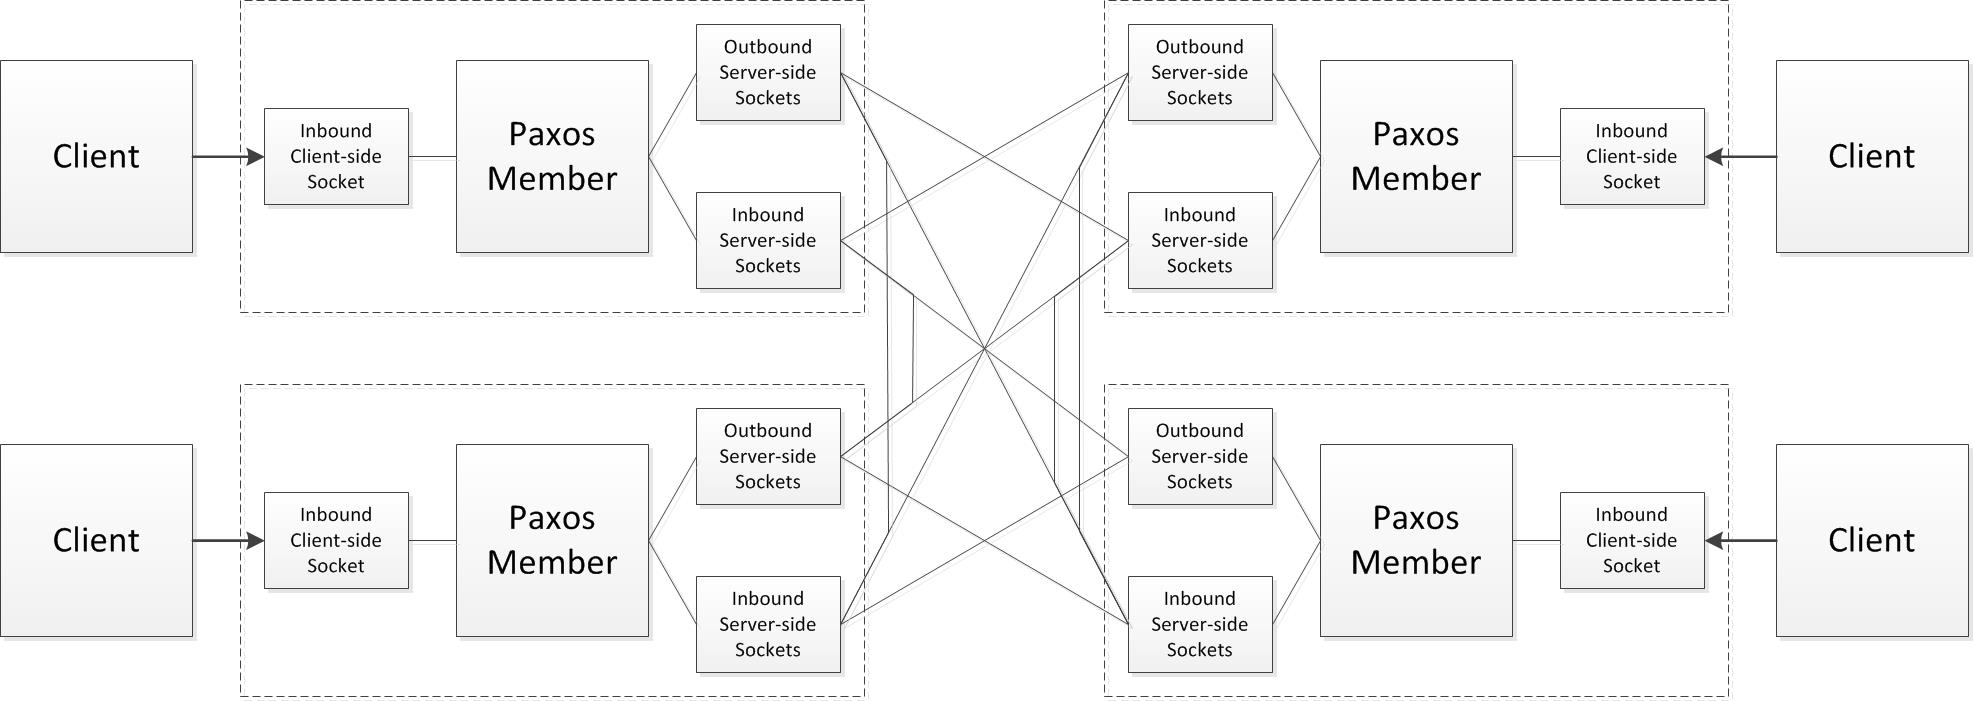
\includegraphics[width=6in]{paxos_group_connections.jpg}
\caption{Paxos Group Connections - each Paxos group member holds connections to clients and connections to communication to every other server in the Paxos group} 
\label{connection_matrix}
\end{figure}

\subsection{Process Architecture}

A server contains one instance of each Paxos role: a proposer, an acceptor, and a learner.
In our implementation, to reduce complexity, we make the proposer also a learner and do not have separate learner entities operating asynchronously in our design on another process.
The combined proposer and learner, and the acceptor run on separate processes for each instance of a server in order to allow each entity to operate asynchronously.
In addition, the combined proposer and learner, and the acceptor each have a message queue which is fed with in-bound messages from other servers and client requests.
These message queues are used to serialize the message streams that may be coming from multiple other server connection processes.

Each server services two different litening server sockets.
Typically, an even numbered port on the server is reserved for listening to client connections while the adjacent higher odd number port is reserved for listening to interserver connections within the Paxos group.
Each inbound connection from other servers first connects to a socket monitored by a listening process say port 9001.
This listening process spawns a new connection process to handle all requests for the newly connected socket on a high port.
Each of these connection processes handle inter-server communication messages and put them on the appropriate message queue bound for the proposer/learner process, or acceptor process depending on the message type.
The proposer process is responsible for opening a client facing socket which allows clients to connect to the service and send request messages.
Proposers handle each connection in a blocking manner where the client connection will block until the requested command issued by the client makes it into an instance of Paxos.
Once a proposer is able to confirm that the command was issued to an instance in the Paxos group, it sends an acknowledgement message back to the client.
The client at this point can either issue another message to trigger another proposal or disconnect singaling the end of the client session.

The process architecture for a single Paxos group member in our implementation running on one server is shown in Figure ~\ref{paxos_member}.

\begin{figure}
\centering
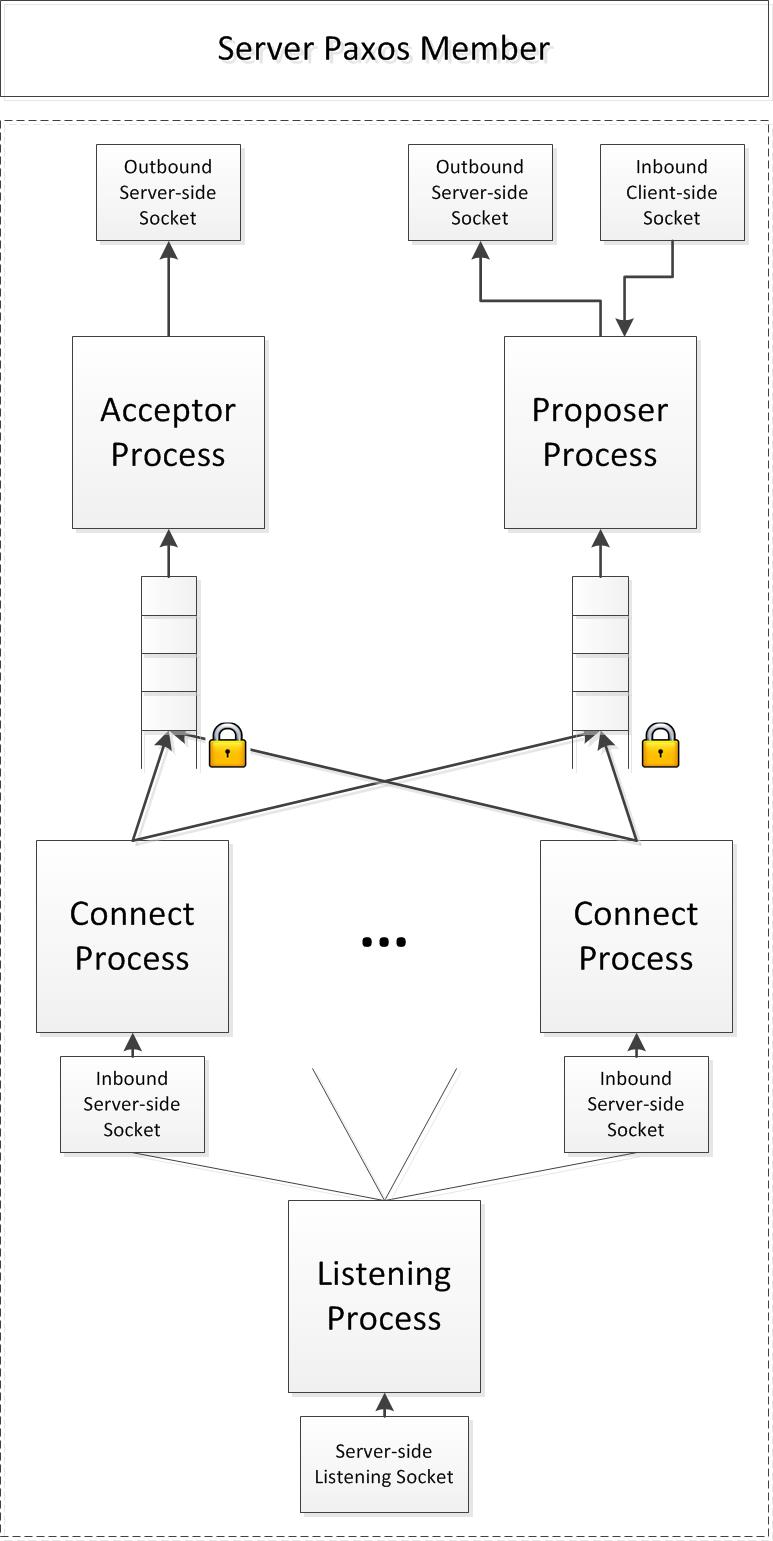
\includegraphics[width=4in]{paxos_member_architecture.jpg}
\caption{Process Architecture - message queues to proposer/learner, and acceptor are serialized; each put() and get() on the message queue is atomic}
\label{paxos_member}
\end{figure}

\subsection{Proposer Finite State Machine}

The proposer executes a finite state machine as summarized in Figure ~\ref{proposer_fsm}.

\begin{figure}
\centering
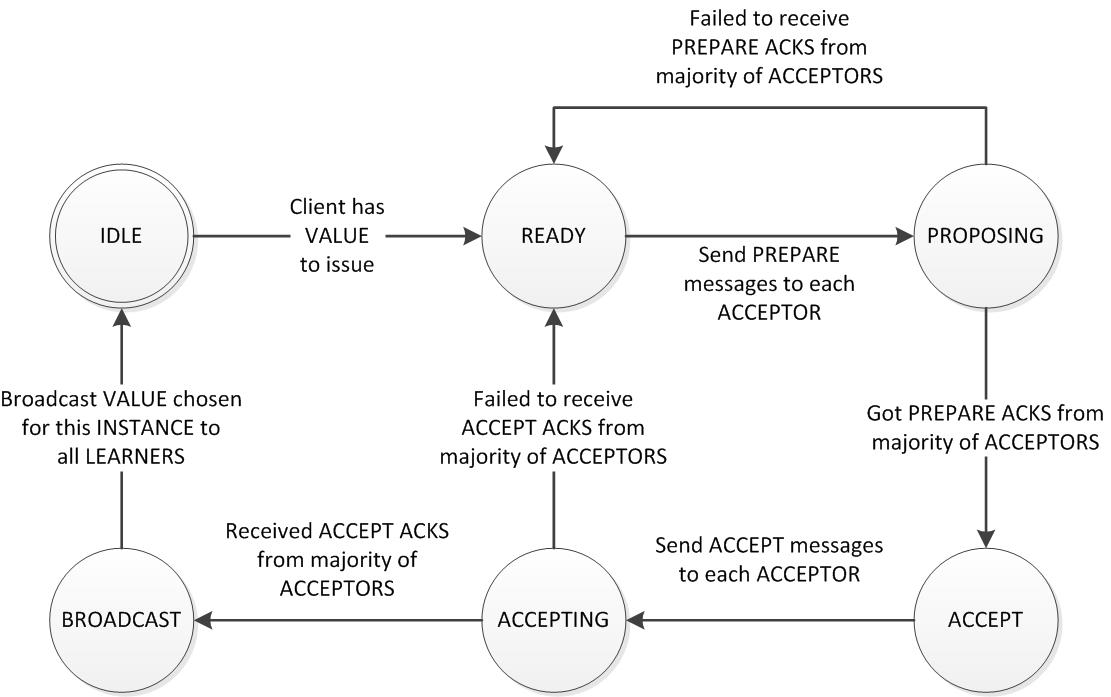
\includegraphics[width=6in]{proposer_fsm.jpg}
\caption{Proposer Finite State Machine}
\label{proposer_fsm}
\end{figure}

State definitions:
\begin{itemize}
\item[IDLE] PROPOSER is waiting for client connection to issue a COMMAND $C_1$ to propose. 
  Upon receiving a COMMAND to propose, a transition to READY is made.
\item[READY] PROPOSER has received a message but no issue proposals to each ACCEPTOR in the Paxos group.
  In this state, the PROPOSER issues PREPARE messages to each ACCEPTOR and unconditionally transitions to the PROPPOSING state.
\item[PROPOSING] PROPOSER has issued PREPARE messages and is waiting for a majority of ACCEPTORS to response with a PREPARE ACK message.
  In this state, if the PROPOSER does not receive a sufficient number of PREPARE ACK messages for its PREPARE request it transitions to the READY state and attempts another proposal.
  If the PROPOSER gets a majority of responses for its original proposer, it moves to the ACCEPT state.
  If the PROPOSER gets a majority of responses that are NACKS for a different value, it moves to the ACCEPT state.
\item[ACCEPT] PROPOSER has received a majority PREPARE ACK or PREPARE NACK for a proposal number and value.
  If in the previous state the PROPOSER received a majority PREPARE ACK messages, it issues an ACCEPT message with the original client COMMAND $C_1$ to each ACCEPTOR in the Paxos group.
  If in the previous state the PROPOSER received a majority PREPARE NACK messages agreeing that a different COMMAND $C_2$ has already been accepted for this instance, it abandons it's original COMMAND $C_1$ as the value of the proposal, and issues this different COMMAND $C_2$ instead as it's accept message.
  An unconditional transition to the ACCEPTING state occurs.
\item[ACCEPTING] PROPOSER has issued ACCEPT requests. 
  If an ACCEPT ACK message is received from a majority of ACCEPTORS, consider the proposal COMMAND determined in the previous state chosen.
  If the chosen command is the original client COMMAND $C_1$, the proposer successfully issued its message and can now go back to the client to ask for new commands and transitions to the IDLE state.
  If the chosen command is not the original client COMMAND $C_1$, the propose failed to issue the client command and must try again be transitioning to the READY state.
  In either case where a command is chosen the proposer learns an instance resolution which is logged in the list of instance resolutions and the instance number for the Paxos member is incremented by one.

  If an insufficient number of ACCEPT ACK message are received after a given time, assume the ACCEPT attempt failed and transition to the READY state to attempt another round.
  In the case where an insufficient number of ACCEPT\_ACK messages are received, the instance number is not incremented because the proposer did not learn an instance resolution and hence it is possible the current instance is not resolved..
\end{itemize}

\subsection{Lock Service Implementation}

The client is implemented such that after sending the server a command message with type CLIENT to request a command be proposed, it will block on a receive from the server until it receives a CLIENT\_ACK message.
If the server receives a CLIENT message, it will block until it has confirmed that the Paxos group has accepted the proposed command into an instance in the Paxos group and that the appropriate lock was acquired or released.
Each client issues a unique client ID field in order to distringuish its requests from other clients which may issue similar requests and to uniquely identify the lock owner.

Because the service for each client is blocking until the request is resolved, in the event of lock contention a client connection will simply wait until the lock has been released and the server it is connected to acquires it on the client's behalf.

In order to ensure that multiple requests for the same lock do not simultaneously get assign in subsequent instances of Paxos, we impose conservative constraints on the conditions for which the instance number may be incremented.
A Paxos proposer may only advance it's instance number to some instance value N if it has learned the values of all instances less than N.
If a value for instance N-1 is not resolved, a proposer must attempt to learn it's value by submitting a proposal to that instance or proposing its own command for issuing.

Though this restriction means that only one instance of Paxos may be resolved at a time and has terrible performance implications, it imposes the guarantee that we will never acquire the same lock simultaneously for two adjacent instances of Paxos (ex. instance N = lock(5), instance N+1 = lock(5)).
It also eliminates the need of a lock broker which introduces additional complexity.

The correctness of the locking service behavior then follows as proposers will necessarily have the correct view of the lock state up to instance N before trying to acquire a lock that is currently held for instance N+1.
If a proposer sees that the lock it wants is currently held, it will wait until the lock is released in a future instance before attempting to acquire it.

It is insufficient simply to block until the lock becomes available as the proposer must issue proposals in order to learn new instance resolutions.
At the same time, the proposer must not cause a lock that is already acquired to be acquired again.
In order to resolve this, we by default attempt to issue the contended lock command for some instance N.
If the instance was already resolved, the proposer should get a majority of PREPARE\_NACKS and be forced to both abandon it's proposal and learn the instance resolution.
The lock set can then be updated before the next proposal.
If the instance has not been resolved but the lock is currently acquired by another member of the Paxos group, the proposer feigns a failure and returns to the READY state after waiting for some amount of time (in our case a second).
By feigning a failure, this guarantees that the contended lock request does not make it to the resolution for this instance.
By waiting for some amount of time, and trying again, it allows other Paxos members to release the lock so that the original requesting member can acquire it in a future instance.
This also indirectly implements a blocking functionality on the client acquisition request.

Once the requested client operation finished, the server issues a message with type CLIENT ACK indicating to the client that the Paxos group successfully accepted the proposal.

The client can then either disconnect from the server, or issue another command to be processed.
Unless the server instance dies or is shutdown, the server never closes the client connection.


%%%%%%%%%%%%%%%%%%%%%%%%%%%%%%%%%%%%%%%%%%%%%%%%%%%%%%%%%%%%%%%%%%%%%%%%%%%%%%
% Instructions for Use
%%%%%%%%%%%%%%%%%%%%%%%%%%%%%%%%%%%%%%%%%%%%%%%%%%%%%%%%%%%%%%%%%%%%%%%%%%%%%%

\section{How to Use Our Implementation}

All of our code can be found in the $\${ROOT_DIR}/src$ folder.
The folder contains a number of unit test files which exercise different aspects of the design.
Each unit test $unittest$ can be executed by simply running $./unittest$ in the $src$ directory.

Unit test files:
\begin{itemize}
\item [acceptor\_test.py] Tests if the client is able to send messages to a dummy server instance, and correctly processes the acknowledgement messages from the server. 
  The dummy server is configured to simply loopback the client request message as an acknowledgement.
\item [acceptor\_test.py] Exercises the acceptor process logic. 
  Creates a dummy server instance for the Paxos acceptor to connect to and injects a sequence of messages into the acceptor process. 
  Response messages are validated and replied to where expected.
\item [proposer\_test.py] Exercises the proposer process logic.
  Creates a dummy server instane for the Paxos proposer to connect to and injects message sequnces to exercise the FSM.
  Response messages are validated and replied to where necessary.
\item [integration\_test.py] Tests basic bring up of a Paxos group with no failures.
  Clients are connected to server instances to verify use cases under the absence of node failures.
\item [failure\_test.py] Tests if the Paxos group still operates correctly under the presence of node failures.
  Server nodes are brought down by terminating all process associated with that server node.
\end{itemize}

To run all tests, in the $src$ directory, issue $make test$.
This should fire off each test case.

%%%%%%%%%%%%%%%%%%%%%%%%%%%%%%%%%%%%%%%%%%%%%%%%%%%%%%%%%%%%%%%%%%%%%%%%%%%%%%
% Known Issues
%%%%%%%%%%%%%%%%%%%%%%%%%%%%%%%%%%%%%%%%%%%%%%%%%%%%%%%%%%%%%%%%%%%%%%%%%%%%%%

\section{Known Issues}

STUB

%%%%%%%%%%%%%%%%%%%%%%%%%%%%%%%%%%%%%%%%%%%%%%%%%%%%%%%%%%%%%%%%%%%%%%%%%%%%%%
% Discussion
%%%%%%%%%%%%%%%%%%%%%%%%%%%%%%%%%%%%%%%%%%%%%%%%%%%%%%%%%%%%%%%%%%%%%%%%%%%%%%

\section{Discussion}

In this section, we discuss a series of potential problems with our implementation of the lock service which we do not resolve, but would have been important considerations should this have been intended to be a production level system.
We also present discussion of

\subsection{Resolving Deadlock}

In our implementation of the lock service, it is entirely possible for deadlock to occur.
The canoncial deadlock scenario is if client A requests locks 1 and 2, while client B requests lock 2 and 1.
If client A is able to acquire lock 1 and client B is able to acquire lock 2, then the system deadlocks.
This particular deadlock stems from a poorly designed lock application and thus we punt this problem to the client application programmer to avoid this sort of deadlock issue.

A second deadlock can occur in the case of orphaned locks.
A lock can be orphaned if a lock command was issued, and the server node failed before it could issue the unlock command associated with the client.
Since each lock acquisition is tagged with a client id, unless the original client comes back online at another server node, no other client may release this lock.
As a result, any other client requesting the orphaned lock is deadlocked.

In order to resolve this issue, we would have needed to implement some sort of watchdog timeout which after a certain period of time proposes to unlock the lock on behalf of the dead client.
This would eventually free up the lock but also does not bypass the Paxos consensus protocol by going through established means to release the lock.

\subsection{Proposal Priority}

In our current implementation, upon initialization, each server is given a unique identifier.
This identifier is made the server's initial proposal number such that proposals from different servers avoid collisions.
However, arbitrarily initializing the proposal number to the server number gives the highest numbered server an unfair advantage.
Thus in the case where all Paxos members are starting a fresh instance simultaneously, the highest numbered proposing server would always ``win'' in that instance.
Since we do not shuffle the initial proposal values after each instance, the highest numbered server will always enjoy a slight advantage over its peers.
To fix this, we would have had to implement a variant of Paxos where a leader token would be rotated among Paxos members such that each member would enjoy highest priority the same number of instances as every other proposer.

\subsection{Optimizing Paxos Instance Resolution}

notes on broadcast

\end{document}
